\chapter{Introduction} \label{intro}
This chapter includes an introduction for AortaGeomRecon assurance cases study. In section \ref{obj}, we are dicussing the objective of this case study, and this documentation. In section \ref{bg}, we are explaning some terms and definitions used throughout this document. Section \ref{ps} discussed about the problem statement, and finally section \ref{TO} gives the brief outline for this document.

%Every thesis needs an introductory chapter
%
%While you're here, you need to go into \texttt{definitions.tex} to set all the 
%information needed for the front matter (e.g. title, author) and page 
%header/footer.
%
%You will also find the School of Graduate Studies' preparation guide (August 
%2021) for theses and reports. I would give it a quick read so you know what's 
%expected.

\section{Objective} \label{obj}
In this study, we present the result of applying of assurance cases in a developing medical software to build the stakeholders' confidence in this software.

\section{Background} \label{bg}
Aorta is the largest artery that carries blood from the heart to the circulatory system. It has a cane-liked shape with Ascending aorta, Aortic arch and Descending aorta. Unlike the real cane stick, the descending aorta might not be straight for each patient. 

\begin{figure}[ht]
    \centering
    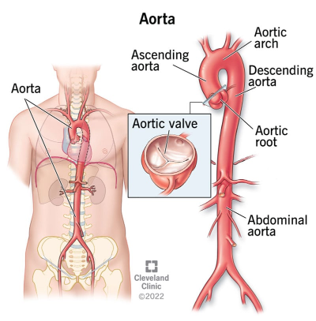
\includegraphics[width=0.7\textwidth]{figures/Sample/Aorta.png}
    \caption[Aorta]{Aorta}
    \label{fig_aorta}
\end{figure}

Aorta segmentation in CT scans is important for:
\begin{itemize}
\item Coarctation of the aorta
\item Aortic calcification quantification
\item To guide the segmentation of other central vessels. 
\end{itemize} ~\\
Assurance cases\\
3D Slicer\\
Image Processing\\

\section{Problem Statement} \label{ps}
The main goals of this project is building a software that can quickly build the 3D geometry of the Aorta from CT Chest scans, while applying the assurance cases for this academic medical software. This project shows the assurance cases can indeed help build up our confidence in the medial software in general, because medical software like real-time system software, needed completeness and correctness.

Build Software and Assurance cases for this software.
Start with a list of Functional and Non-Functional requirements.

\section{Thesis Outline} \label{TO}
